%%%%%%%%%%%%%%
% LECTURE 20 %
%%%%%%%%%%%%%%
\vspace{1cm}

\noindent\lecture{20}{17/12/2021}
\section{Sistemi superconduttivi}
Dopo aver studiato e analizzato i sistemi a trappola ionica, diamo uno sguardo, in maniera del tutto generale, a un altro modo, molto diffuso e utilizzato, di andare a realizzare sistemi a due livelli: i \textbf{sistemi superconduttivi}. Spesso vengono anche definiti come \textbf{circuiti QED} (\textbf{cQED}) in analogia proprio con le cavità QED (CQED). Negli esempi analizzati nel caso della CQED si sfruttava il fatto che un semplice modello possa essere utilizzato per descrivere l'interazione di un atomo con una cavità ottica oppure anche per spiegare l'accoppiamento di un qubit con un risonatore a microonde: questo modello include il numero di fotoni nella cavità/risonatore, lo stato dell'atomo/qubit e l'interazione del dipolo elettrico tra l'atomo/qubit e la cavità/risonatore.

\noindent Invece, come suggerisce il nome, la fisica che sta dietro ai sistemi superconduttivi sfrutta il fenomeno della superconduttività. Per una trattazione completa sarebbe richiesto un corso intero, per cui, nel nostro studio, ci limitiamo a riportare i risultati generali che serviranno a descrivere questo tipo di sistemi.

\subsection{Cenni di superconduttività}

L'idea alla base della realizzazione fisica dei qubit è abbastanza semplice, tuttavia la fisica che ci sta dietro è abbastanza complessa perché coinvolge il concetto della \textbf{superconduttività}. Prima di vedere come si realizza la costruzione dei qubit e dei gate, facciamo alcuni cenni su questo importante argomento. 

\noindent Che cos'è la superconduttività? In corrispondenza di temperature sufficientemente basse, elementi metallici ed alcuni semiconduttori vanno incontro ad una transizione di fase. Al di sotto di una particolare temperatura, detta temperatura critica $T_C$, essi acquistano notevoli proprietà fisiche; la loro resistività
diventa bruscamente nulla, perciò in questi materiali diventa possibile, in assenza di campi esterni, misurare correnti che non decadono nel tempo. L’assenza di effetti dissipativi nel meccanismo di conduzione, assieme ad altri fenomeni correlati, sono indicati sinteticamente con il termine \textbf{superconduttività}. Nel 1957 J. Bardeen, L. N. Cooper e J. R. Schrieffer, formularono la prima teoria microscopica della superconduttività (\textbf{teoria BCS}) utilizzando la meccanica quantistica, che valse loro il Nobel nel 1972. Tale teoria è in grado di dare una spiegazione del fenomeno della superconduzione (capacità predittiva e base per le applicazioni). 

\noindent Il fenomeno della superconduttività consiste nella creazione, per mezzo dello scambio di fononi nel metallo e a temperatura sufficientemente bassa, di stati legati costituiti da coppie di elettroni $(e^-,e^-)$, chiamate \textbf{coppie di Cooper}. Questi oggetti sono ovviamente bosoni e costituiscono un particolare condensato di Bose-Einstein.

\noindent In questa configurazione, mentre i fermioni, a causa del principio di esclusione di Pauli, sono disposti in maniera tale da non avere lo stesso set di numeri quantici, i bosoni, a basse temperature, sono tutti situati nello stato fondamentale. In un metallo regolare se gli elettroni vengono messi in moto, tipicamente, per via della presenza di impurezze o reticoli di cristallo con cui gli elettroni fanno scattering, vi è una resistenza. La stessa situazione vale per i bosoni, ma vi è una interazione di scambio: è energicamente favorevole mettere i bosoni nello stesso stato (stesso set di numeri quantici), in particolare nello stato fondamentale perché per spostare uno di questi bosoni è richiesta una grande quantità di energia. La corrente che si viene a originare è un flusso di bosoni, tutti con la stessa velocità e dato che è richiesta energia per rimuovere un bosone dallo stato in cui si trovano tutti gli altri, hanno tutti una bassa resistenza. Un esempio di spettro energetico a basse temperature di un materiale superconduttivo è dato dalla Figura \ref{fig:super-spectrum}.

\begin{figure}[!ht]
    \centering
    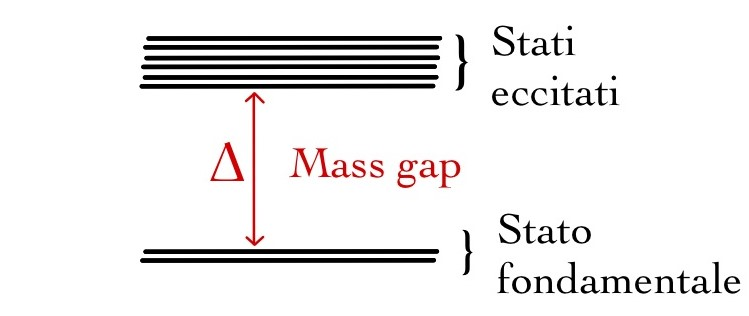
\includegraphics[scale=0.45]{images/super-spectrum.jpg}
    \caption{Spettro energetico di un materiale superconduttivo. La differenza tra lo stato fondamentale e gli stati eccitati è noto come \textbf{mass gap} $\Delta$.}
    \label{fig:super-spectrum}
\end{figure}


\subsection{cQED}

L'idea è quella di realizzare dei qubit con dei piccoli circuiti superconduttivi (non si tratta più di un sistema atomico o di spin). Un tale sistema sembrerebbe a prima vista macroscopico, tuttavia, come vedremo, grazie alla presenza del fenomeno della superconduttività è davvero quantistico. 

\begin{figure}[H]
    \centering
    \begin{circuitikz}
        \draw
        (0,0)   to[C=$C$] ++ (0, 2) -- ++ ( 2,0) 
                to[L=$L$] ++ (0,-2) -- ++ (-2,0)
                (1,0)node[ground]{};
    \end{circuitikz}
    \caption{Circuito LC.}
    \label{fig:lc-circuit}
\end{figure}

\noindent Ancora una volta si utilizza un oscillatore armonico: affinché si possa utilizzare come un sistema a due livelli è necessario introdurre dell'anarmonicità nei livelli energetici così da poter distinguere lo stato fondamentale dal primo eccitato senza preoccuparsi degli altri livelli. Il nostro punto di partenza è un semplice \textbf{circuito LC}, come mostrato in Figura \ref{fig:lc-circuit}.

\noindent Vediamo il motivo per cui un tale circuito presenta un comportamento oscillatorio. Innanzitutto, ricordiamo che ciascun elemento mette in relazione la carica o la corrente con il potenziale; in particolare le relazioni costitutive della capacità e dell'induttanza risultano:
\begin{align*}
    &\text{Capacità:} &Q & =CV\, , \\
    &\text{Induttanza:} &V &= L\dv{I}{t}\, .
\end{align*}
Per svolgere questo tipo di trattazione può tornare utile riscrivere la corrente come $I=\dv{Q}{t}$ e introdurre il \textit{flusso} definito come
\begin{equation*}
    \Phi(t)=\int_{-\infty}^{t} \dd{t'} V(t') \, ;
\end{equation*}
a questo punto, la relazione sull'induttanza può, ad esempio, essere riscritta in termini di flusso integrando entrambi i membri 
\begin{equation*}
    \Phi = LI \, .
\end{equation*}
Note le relazioni tra carica/corrente e potenziale, possiamo andare a valutare le energie associate a ciascun elemento del circuito. A partire da
\begin{equation}\label{eq:general-energy}
    E(t)=\int_{-\infty}^{t} \dd{t'} V(t')I(t') \quad (\text{da } \delta E = V \delta Q) \, ,
\end{equation}
assumendo che tutte le quantità in gioco si annullino a $t=-\infty$, ricaviamo
\begin{align*}
    &\text{Capacità:} &E&=\int_{-\infty}^{t} \dd{t'} VC\derivative{V}{t'}=\frac C 2 V^2 = \frac{Q^2}{2C} \, , \\
    &\text{Induttanza:} &E&=\int_{-\infty}^{t} \dd{t'} L\derivative{I}{t'}I=\frac L 2 I^2 \equiv \frac{\Phi^2}{2L}\, .
\end{align*}
In una trattazione classica possiamo interpretare il termine relativo alla capacità come un'\textbf{energia cinetica} mentre quello relativo all'induttanza come \textbf{energia potenziale}. In questo contesto possiamo andare a scrivere la lagrangiana classica del sistema nel seguente modo
\begin{align*}
    \mathcal{L}&= E_k - E_p = \frac{Q^2}{2C}-\frac{\Phi^2}{2L} = \frac{C}{2}V^2-\frac{\Phi^2}{2L} = \frac{C}{2}\dot{\Phi}^2-\frac{\Phi^2}{2L} \, ,
\end{align*}
dove abbiamo inserito il fatto che $V = \dv{\Phi}{t}$. Applicando le equazioni di Eulero-Lagrange
\begin{equation*}
    \dv{t} \left(\pdv{\mathcal{L}}{\dot{\Phi}}\right)-\pdv{\mathcal{L}}{\Phi}=0 \, ,
\end{equation*}
si ottiene l'equazione del moto
\begin{equation*}
    C\ddot{\Phi}+\frac{\Phi}{L}=0 \, ,
\end{equation*}
che possiamo riscrivere sotto forma di equazione del moto di un oscillatore armonico nel seguente modo
\begin{equation*}
    \ddot{\Phi}+\omega^2\Phi = 0 \, , \quad \text{con} \quad \omega=\frac{1}{\sqrt{LC}} \, .
\end{equation*}
Per passare ad una descrizione quantistica del sistema dobbiamo riscrivere la fisica nel formalismo hamiltoniano. Calcoliamo il \textit{momento coniugato}
\begin{equation*}
    \Pi = \fdv{\mathcal{L}}{\dot{\Phi}} = C\dot{\Phi} = CV = Q\, ,
\end{equation*}
cosicché possiamo calcolarci la \textit{trasformata di Legendre} della lagrangiana precedente
\begin{equation}\label{eq:ham-LC}
        H = \Pi\dot{\Phi} - \mathcal{L} = Q\frac QC - \left(\frac{Q^2}{2C}-\frac{\Phi^2}{2L}\right) = \frac{Q^2}{2C} + \frac{\Phi^2}{2L} \, ;
\end{equation}
è evidente che l'hamiltoniana corrisponde proprio alla somma dell'energia cinetica e dell'energia potenziale.

\noindent Supponiamo ora di considerare il medesimo sistema, ma di volerne dare una descrizione quantistica. In Tabella \ref{tab:oa-lc} sono riportate le relative identificazioni con il nuovo sistema quantistico.
\begin{table}[H]
	\centering
    \begin{tabular}{c|c}
        \toprule
        Oscillatore armonico & Circuito LC \\
        \midrule
        $H=\frac{\hat{p}^2}{2m}+\frac{m}{2}\omega^2\hat{x}$ & $H=\frac{Q^2}{2C}+\frac C2 \omega^2\Phi^2$ \\
        \midrule
        $\hat{x}$ & $\Phi$ \\
        \hline
        $\hat{p}$ & $Q$ \\
        \hline
        $m$ & $C$ \\
        \bottomrule
    \end{tabular}\\
    \caption{Identificazioni tra quantità fisiche e operatori dell'oscillatore armonico quantistico e le grandezze fisiche di un circuito LC. Si ricordi che per il circuito LC la frequenza è $\omega = \frac{1}{\sqrt{LC}}$.}
    \label{tab:oa-lc}
\end{table}
\noindent Possiamo quindi mappare un circuito LC con un oscillatore armonico e imporre la quantizzazione canonica per quantizzare un tale sistema. Possiamo promuovere $(\Phi, Q) \to (\hat{\Phi}, \hat{Q})$ ad operatori e scriverli in funzioni degli operatori di creazione e distruzione
\begin{equation}\label{Phi_Q_oscill}
    \hat \Phi = \sqrt{\frac{\hbar}{2C\omega}}\left(\hat a + \hat a^\dagger\right) \, , \qquad \hat Q = \frac{\sqrt{2C \omega \hbar}}{2i}\left(\hat a - \hat a^\dagger\right) \, ;
\end{equation}
in questo modo imponiamo le seguenti regole di commutazione
\begin{equation*}
    \comm{\hat \Phi}{\hat Q}=i\hbar \, , \quad \Leftrightarrow \quad \comm{\hat a}{\hat a^\dagger}=1 \, .
\end{equation*}
È dunque evidente che la procedura di quantizzazione è immediata, tuttavia è abbastanza insolito pensare di svolgere una trattazione quantistica di un sistema macroscopico. 
\noindent Se supponiamo invece di considerare un sistema superconduttivo, possiamo utilizzare alcuni risultati della teoria BCS per riscrivere l'hamiltoniana della relazione \eqref{eq:ham-LC} nel seguente modo
\begin{equation}\label{eq:ham-oa-cQED}
    \hat H = 4E_C\hat n^2 + \frac{E_L}{2}\hat \phi^2 \, , \quad \text{con} \quad \hbar\omega=\sqrt{8E_LE_C} \, ,
\end{equation}
dove
\begin{itemize}
    \item $\hat n = \frac{Q}{2e}$ è l'operatore che indica il numero di coppie di Cooper;
    \item $\hat \phi = \frac{2\pi}{\Phi_0}\Phi$ è l'operatore del flusso ridotto ($\Phi_0=\frac{h}{2e}$ è il \textit{quanto di flusso});
    \item $E_C=\frac{e^2}{2C}$ è l'energia necessaria per aggiungere un elettrone extra alla capacità del circuito;
    \item $E_L=\left(\frac{\Phi_0}{2\pi}\right)^2\frac 1 L$ è l'energia associata all'induttanza.
\end{itemize}
L'altro fatto fondamentale, accanto all'utilizzo di materiali superconduttivi, che rende il sistema adatto ad una descrizione quantistica è che in realtà non andiamo a utilizzare un circuito LC generico (il quale presenta infiniti livelli energetici equidistanti), ma uno in cui si introduce una cosiddetta \textbf{giunzione Josephson} (Figura \ref{subfig:JJ-circuit}). Quest'ultima produce il cosiddetto \textbf{effetto Josephson} (Figura \ref{subfig:J-effect}),  introducendo quindi dell'anarmonicità. 

\begin{figure}[!ht]
	\centering	
	\subfloat[][\label{subfig:JJ-circuit}]{
	    \begin{circuitikz}
        \draw
        (0,0)   to[C=$C$] ++ (0, 2) -- ++ ( 2,0) 
                to[josephson=$L$] ++ (0,-2) -- ++ (-2,0)
                (1,0)node[ground]{};
    \end{circuitikz}
	} \qquad
	\subfloat[][\label{subfig:J-effect}]{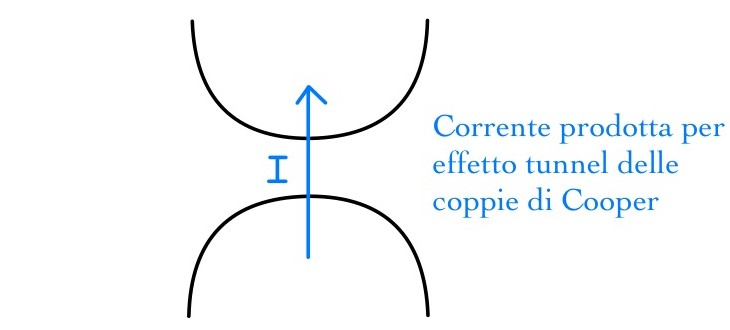
\includegraphics[scale=.4,keepaspectratio]{images/J-effect.jpg}}
	\caption{(\ref{subfig:JJ-circuit}) Circuito LC con giunzione Josephson (la giunzione è caratterizzata da una propria capacità $C_J$ e induttanza $L_J$). D'ora in avanti indicheremo nei circuiti una giunzione Josephson con la notazione di questo circuito. (\ref{subfig:J-effect}) Effetto tunnel della coppia di Cooper tra due elettrodi metallici superconduttivi sufficientemente vicini e separati da una sottile barriera di ossido.}
\end{figure}
\noindent L'effetto Josephson può essere riassunto nei seguenti due risultati:
\begin{enumerate}
    \item La corrente prodotta per effetto tunnel delle coppie di Cooper segue la \textbf{prima legge di Josephson}
    \begin{equation}\label{1_Josephson_law}
        I = I_C \sin \phi \, ,
    \end{equation}
    dove $I_C$ è detta \textbf{corrente critica};
    
    \item Applicando una differenza di potenziale ai capi degli elettrodi scorrerà un'altra corrente, la quale segue la \textbf{seconda legge di Josephson}
    \begin{equation}\label{2_Josephson_law}
        V = \dv{\Phi}{t} = \frac{\hbar}{2 e} \dv{\phi}{t} \, .
    \end{equation}
\end{enumerate}
Se si costruisce un circuito LC inserendo questa giunzione è possibile ricalcolare l'energia potenziale associata al circuito sfruttando la relazione in \eqref{eq:general-energy} 
\begin{equation}\label{eq:E_Josephson}
    E=\int_{-\infty}^{t} \dd{t'} V(t')I(t')=\frac{\hbar}{2e}I_C\int_{-\infty}^{t} \dd{t'} \derivative{\phi}{t'}\sin\phi =-E_J\cos\phi \, ,
\end{equation}
dove abbiamo indicato l'\textbf{energia Josephson} con $E_J = \frac{\hbar I_C}{2e}$. In questo modo l'hamiltoniana di un sistema di questo tipo risulta in
\begin{equation}\label{eq:ham-jj}
    \hat H = 4E_C\hat n^2-E_J\cos\hat \phi \, ,
\end{equation}
che differisce dalla \eqref{eq:ham-oa-cQED} per la presenza di un potenziale periodico anarmonico. In Figura \ref{fig:jj-spectrum} si può osservare lo spettro energetico dell'hamiltoniana che descrive un circuito LC con giunzione Josephson. L'obiettivo è quello di utilizzare per la costruzione di un qubit i livelli energetici evidenziati in figura: il punto fondamentale è stato l'introduzione della giunzione Josephson, la quale non solo rende il sistema veramente quantistico, ma soprattutto introduce dell'anarmonicità nello spettro dell'oscillatore. 

\begin{figure}[!ht]
    \centering
    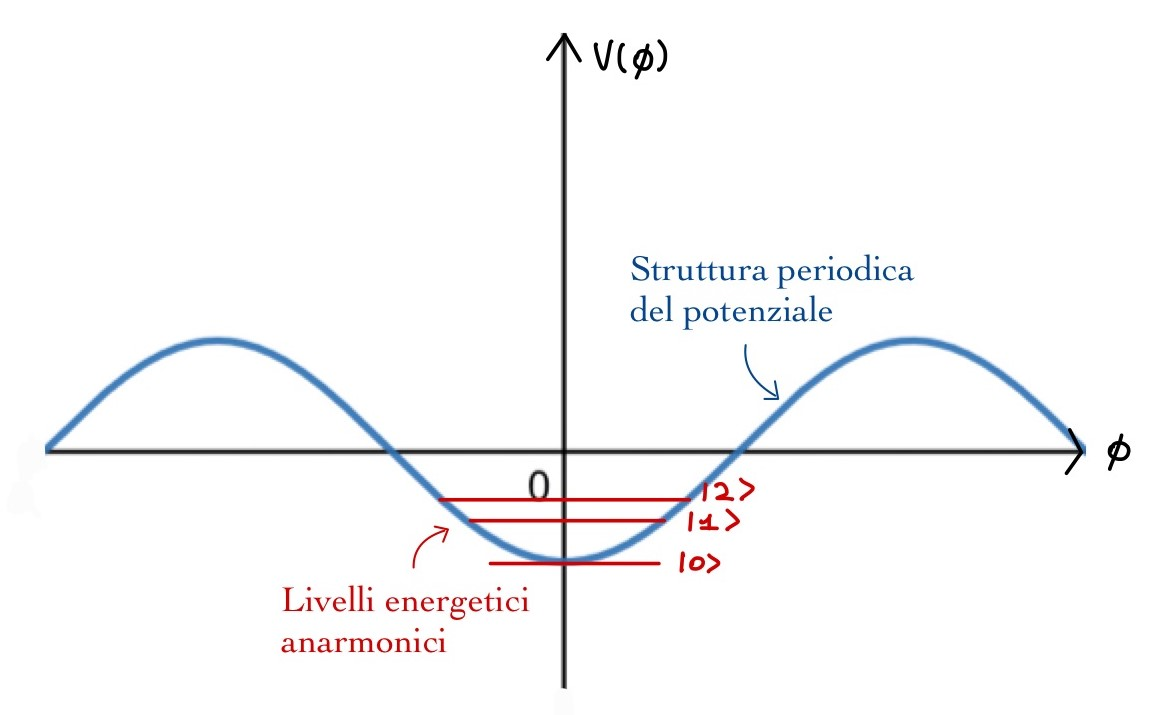
\includegraphics[scale=0.35]{images/jj-spectrum.jpg}
    \caption{Spettro energetico dell'hamiltoniana in \eqref{eq:ham-jj}. Per piccoli $\phi$ possiamo approssimare lo spettro come dei livelli energetici dell'oscillatore armonico più piccole correzioni anarmoniche.}
    \label{fig:jj-spectrum}
\end{figure}


\subsection{Interpretazione dell'effetto Josephson}
Per parlare in maniera del tutto completa ed esaustiva dell'effetto Josephson sarebbe necessaria una lezione completa, pertanto per approfondimenti e chiarimenti rimandiamo a corsi sulla superconduttività. 

\noindent L'idea che seguiamo è quella di procedere attraverso una trattazione schematica dell'effetto Josephson dovuta a Feynman. Il punto di partenza è la differenza nello spettro energetico che c'è tra un metallo normale, dove possiamo avere bande che sono riempite da un mare di elettroni (Figura \ref{subfig:metal-energy-spectrum}) e un superconduttore, in cui vi è una netta separazione tra lo stato fondamentale e gli stati eccitati (Figura \ref{subfig:superconductor-energy-spectrum}). 

\noindent Nel momento in cui andiamo a considerare una giunzione metallica come in basso in Figura \ref{subfig:metal-energy-spectrum}, costituita da due elettrodi ciascuno con il proprio mare di elettroni riempito fino all'energia di Fermi $\varepsilon_F$, e supponiamo che tra i due vi sia una differenza di potenziale $V$, allora possiamo osservare una corrente $I$ che scorre tra i due terminali dovuta al fatto che gli elettroni possano fare tunneling da un elettrodo a un altro. Questa corrente $I$ sarà proporzionale alla tensione applicata $V$ e il coefficiente di proporzionalità è dato dall'inverso della resistenza $R$ del sistema. Supponiamo invece di considerare due metalli superconduttivi, che indichiamo con (L) left e (R) right, ciascuno caratterizzato da un mass-gap $\Delta$: a basse temperature, dove la fisica della superconduttività è rilevante, quello che succede è che gli stati fondamentali di entrambi saranno occupati da un certo numero di coppie di Cooper $N_L$ e $N_R$; in tale situazione il tunneling è dovuto alle coppie di Cooper, da sinistra verso destra e viceversa.

\begin{figure}[!ht]
	\centering	
	\subfloat[][\label{subfig:metal-energy-spectrum}]{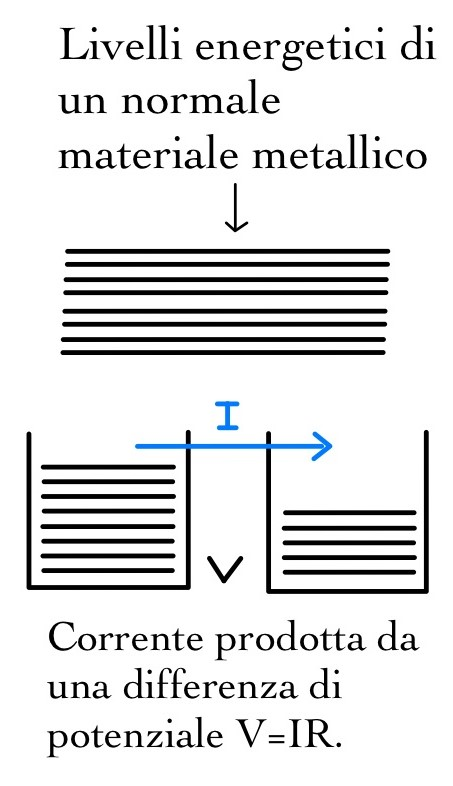
\includegraphics[scale=.3,keepaspectratio]{images/metal-energy-spectrum}} \qquad \qquad
	\subfloat[][\label{subfig:superconductor-energy-spectrum}]{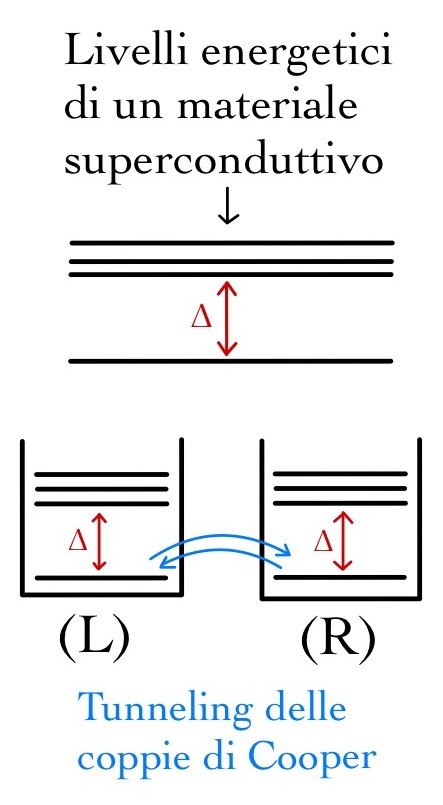
\includegraphics[scale=.3,keepaspectratio]{images/superconductor-energy-spectrum}} \qquad
	\caption{(\ref{subfig:metal-energy-spectrum}) Livelli energetici di un metallo caratterizzato da un mare di elettroni e sistema di due elettrodi in cui avviene il fenomeno del tunneling di elettroni da un elettrodo all'altro. (\ref{subfig:superconductor-energy-spectrum}) Livelli energetici di un metallo superconduttivo caratterizzato, a basse temperature, da uno stato fondamentale in cui si trovano tutte le coppie di Cooper e i livelli eccitati separati da un mass-gap $\Delta$ e sistema di due elettrodi superconduttivi in cui avviene il fenomeno del tunneling di coppie di Cooper da un elettrodo all'altro.}
\end{figure}

\noindent Dal punto di vista della QM, se la temperatura è sufficientemente bassa a tal punto da non considerare gli stati eccitati, ciò che conta è il numero quantico che identifica quanti bosoni sono nello stato fondamentale. Nel nostro caso, il sistema dei due elettrodi superconduttivi è descritto da due interi $N_L$ e $N_R$ (numero di coppie di Cooper nello stato fondamentale presenti rispettivamente nell'elettrodo di sinistra e nell'elettrodo di destra). Passare da un elettrodo all'altro significa quindi andare a incrementare e diminuire il numero di bosoni di entrambi gli elettrodi: ad esempio
\begin{equation*}
    \substack{\text{Tunneling di} \\ \text{un bosone da} \\ \text{(L) a (R)}}: \quad \ket{N_L, N_R} \longrightarrow \ket{N_L-1, N_R+1}
\end{equation*}
Dal momento che il numero totale di bosoni dei due elettrodi è fissato, è sufficiente analizzare solamente uno di questi due numeri, ad esempio $N_L$ e lo andiamo a identificare con $m$ e il corrispondente stato con $\ket m$, cioè il numero di coppie di Cooper nel primo metallo. L'idea di Feynman è quella di andare a modellizzare il tunneling tramite un'hamiltoniana di interazione che non è altro che una matrice $2 \times 2$:
\begin{equation*}
    \hat H = -\frac{E_J}{2}\sum_m\big(\underbrace{\op{m}{m+1}}_{\substack{\text{Operatore che} \\ \text{riduce il numero} \\ \text{di coppie} \\ \text{di Cooper.}}}+\underbrace{\op{m+1}{m}}_{\substack{\text{Operatore che} \\ \text{incrementa il} \\ \text{numero di coppie} \\ \text{di Cooper.}}}\big) \, .
\end{equation*}
Questa hamiltoniana è caratterizzata da due operatori che non fanno altro che eseguire il tunneling di una coppia di Cooper da un metallo superconduttivo all'altro. Da questa definizione si possono ottenere vari risultati che ci limitiamo a citare, ma che possono essere verificati con semplici conti di QM:
\begin{enumerate}
    \item Gli autostati dell'hamiltoniana precedente sono del tipo
    \begin{equation*}
        \ket{\varphi}=\sum_{m=-\infty}^{+\infty}e^{im\varphi}\ket{m} \, , \quad \text{con} \quad \varphi \in [0,2\pi) \, ,
    \end{equation*}
    e gli autovalori sono dati dall'energia nella \eqref{eq:E_Josephson} 
    \begin{equation*}
        \hat H \ket{\varphi} = -E_J \cos\varphi\ket{\varphi} \, ,
    \end{equation*}
    dove si vede che il flusso ridotto $\phi$ pu\`o essere identificato con la fase $\varphi$ degli autostati.
    \item Definendo un operatore numero $\hat n$ che indica il numero di coppie di Cooper trasferite attraverso la giunzione
    \begin{equation*}
        \hat n = \sum_m m\op{m}{m} \, ,
    \end{equation*}
    cioè tale che
    \begin{equation*}
        \hat n \ket m = m \ket m \, ;
    \end{equation*}
    e definendo inoltre un operatore corrente $\hat{I}$ tale che
    \begin{equation*}
        \hat{I} = 2 e \dv{\hat{n}}{t} = \frac{2 i e}{\hbar} \comm{\hat{H}}{\hat{n}} -i\frac{e}{\hbar}E_J\sum_m\op{m}{m+1}-\op{m+1}{m} \, ,
    \end{equation*}
    allora è possibile ottenere la prima legge di Josephson della \eqref{1_Josephson_law}
    \begin{equation*}
        \hat I \ket{\varphi} = \underbrace{\frac{2eE_J}{\hbar}}_{I_C} \sin\varphi \ket\varphi = I_C \sin\varphi \ket{\varphi} \, .
    \end{equation*}
    
    
    \item Cosa succede quando si applica una differenza di potenziale tra gli elettrodi dei metalli? Pensiamo alla situazione in cui un campo elettrico esterno viene applicato e mantenuto in modo tale che vi sia una caduta di tensione fissa $V$ attraverso il tunnel della giunzione. Questo modifica l'hamiltoniana nel seguente modo
    \begin{equation*}
        \hat H \longrightarrow \hat H -(2e)V\hat n \, ;
    \end{equation*}
    si tratta di un esercizio di QM dimostrare che l'evoluzione temporale dello stato a seguito dell'equazione di Schr\"odinger non è altro che 
    \begin{equation*}
        \ket{\psi(t)}=\exp{\frac{i}{\hbar}E_J\int_0^t\dd{\tau}\cos\left(\varphi(0)+\frac{2e}{\hbar}V\tau\right)}\ket{\varphi_0+\frac{2e}{\hbar}Vt} \, .
    \end{equation*}
    Dunque partendo al tempo $t=0$ dallo stato $\ket{\psi(0)} = \ket{\varphi_0}$, allora al tempo $t$ si ottiene una fase globale e lo stato evolve linearmente nel tempo risultando shiftato di $\varphi_0 \to \varphi_0 + \frac{2 e V}{\hbar} t$. Questo significa che riotteniamo la seconda legge di Josephson della \eqref{2_Josephson_law} usando ancora $\varphi=\phi$
    \begin{equation*}
        \dv{\phi}{t} = \frac{2 e V}{\hbar} \, , \quad \Rightarrow \quad V = \frac{\hbar}{2 e} \dv{\phi}{t} \, . 
    \end{equation*}
\end{enumerate}

\noindent Per riassumere, ciò di cui abbiamo bisogno sono le seguenti informazioni: la natura quantistica del sistema è data dallo stato fondamentale, il quale è l'unico che importa nella superconduttività; la corrente che si origina è dovuta al tunneling delle coppie di Cooper, le quali sono frutto di una particolare condensazione di bosoni; l'oscillatore risultante è quantistico, ma non armonico perché l'hamiltoniana associata è data dalla relazione \eqref{eq:ham-jj}. 

\subsection{Transmon qubit}
Discutiamo come codificare un qubit in un circuito come quello di Figura \ref{subfig:J-effect}. Tra tutte le varie tipologie di qubit superconduttivi, quello più popolare e largamente utilizzato è il regime del cosiddetto \textbf{transmon qubit}. Consideriamo l'hamiltoniana ottenuta in \eqref{eq:ham-jj} a cui aggiungiamo un termine costante $E_J$ (questo porta a una variazione nei livelli energetici, ma non sulla dinamica del sistema)
\begin{equation*}
    \hat H = 4E_C\hat n^2 + E_J(1-\cos\hat\phi) \, .
\end{equation*}

\noindent I transmon qubit si hanno nel limite in cui $E_J/E_C \gg 1$, ossia quando $\phi \sim 0$. Questo limite ci permette di sviluppare il potenziale attraverso un'espansione con il polinomio di Taylor
\begin{equation*}
    \hat V(\hat \phi)=E_J(1-\cos\hat \phi)=\frac{E_J}{2!}\hat \phi^2-\frac{E_J}{4!}\hat \phi^4 + \frac{E_J}{6!}\hat \phi^6 + \order{\hat\phi^8} \, ;
\end{equation*}
si noti che il primo termine genera il potenziale armonico. Per capire il peso relativo di ciascun termine è utile normalizzare il primo introducendo il cambio di variabili $\hat x=\sqrt{E_J}\hat \phi$:
\begin{equation*}
    \hat V(\hat \phi)= \frac{\hat x^2}{2}-\frac{\hat x^4}{4!E_J}+\frac{\hat x^6}{6!E_J^2} + \order{\hat{x}^8} \, ;
\end{equation*}
i vari termini sono soppressi da potenze di $E_J$. Se tronchiamo l'espansione al termine di ordine $\hat{x}^4$, l'hamiltoniana del transmon qubit risultante sarà
\begin{equation}\label{eq:ham-transmon}
    \hat H = \underbrace{4E_C\hat n^2 + \frac{E_J\hat \phi^2}{2}}_{\hat H_0}\underbrace{-\frac{E_J\hat\phi^4}{24}}_{\text{correzione}} \, ,
\end{equation}
dove si è indicato con $\hat{H}_0$ la corrispondente hamiltoniana di oscillatore armonico. In Figura \ref{fig:ho-transmon} sono riportate le differenze nello spettro di un oscillatore armonico (Figura \ref{subfig:ho-transmon1}) e un oscillatore anarmonico con \textbf{accoppiamento quartico} (Figura \ref{subfig:ho-transmon2}), dovuto al termine chiamato \textit{correzione}.

\begin{figure}[H]
	\centering	
	\subfloat[][\label{subfig:ho-transmon1}]{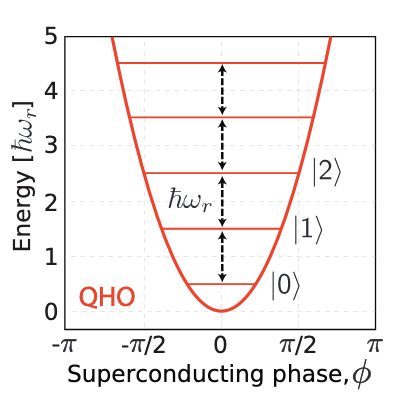
\includegraphics[scale=.8,keepaspectratio]{images/ho-transmon1.jpg}} \qquad \qquad
	\subfloat[][\label{subfig:ho-transmon2}]{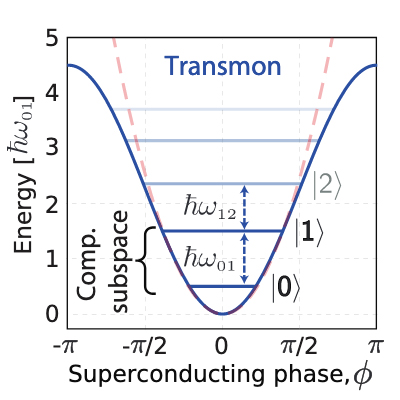
\includegraphics[scale=.8,keepaspectratio]{images/ho-transmon2.jpg}}
	\caption{(\ref{subfig:ho-transmon1}) Spettro energetico del QHO, dove i livelli di energia sono equidistanti l'uno dall'altro. (\ref{subfig:ho-transmon2}) La giunzione Josephson rimodella il potenziale energetico quadratico (tratteggiato in rosso) in sinusoidale (blu fisso), il quale non presenta più livelli energetici equispaziati. Si noti che questo potenziale è una buona approssimazione solamente nel limite $\phi \simeq 0$.}
	\label{fig:ho-transmon}
\end{figure}

\noindent In questa nuova configurazione gli autovalori non sono più equidistanziati: in Figura \ref{fig:energy-difference-transmon} possiamo notare che gli stati $\ket 0$ e $\ket 1$ sono separati da un'energia $\hbar\omega$, mentre gli stati $\ket 1$ e $\ket 2$ da un'energia $\hbar\omega+\alpha$ con $\alpha<0$. (Si veda la discussione che segue per capire perché in figura è indicata la frequenza "$\tilde{\omega}$", non "$\omega$"). 

\begin{figure}[H]
	\centering	
	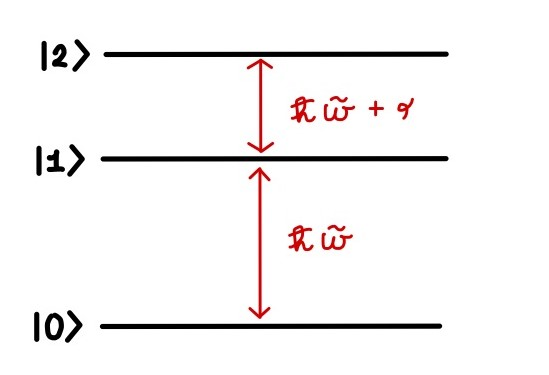
\includegraphics[scale=.45, keepaspectratio]{images/energy-difference-transmon.jpg}
	\caption{Differenza energetica tra i livelli $\ket 0$, $\ket 1$ e $\ket 2$.}
	\label{fig:energy-difference-transmon}
\end{figure}

\noindent Se $\hbar \omega$ è ragionevolmente grande possiamo pensare di utilizzare gli stati $\ket{0}$ e $\ket{1}$ per codificare il qubit e usare degli impulsi laser esterni di frequenza $\sim \omega$ per mandare solamente $\ket{0} \leftrightarrow \ket{1}$, dato che questi livelli non sono in risonanza con tutti gli altri. In particolare, nel caso dei transmon qubit, si lavora con $\omega \sim 3-4 \text{ GHz}$ mentre $\alpha \sim 300 \text{ MHz}$, quindi $E_J/E_C \sim 40$. Tuttavia, a volte, per misure di precisione, si necessita l'utilizzo del livello $\ket 2$, quindi non lo si tiene molto distante energeticamente dagli altri livelli.

\noindent Per vedere esplicitamente come avviene la codifica del qubit, usiamo la definizione di $\hat \phi$ e esplicitiamo gli oscillatori delle relazioni \eqref{Phi_Q_oscill}
\begin{align*}
    \hat \phi = \frac{2\pi}{\Phi_0}\Phi = \frac{2e}{\hbar}\Phi = \frac{2e}{\hbar}\sqrt{\frac{\hbar}{2C\omega}}\left(\hat a + \hat a^\dagger\right) = 2\left(\frac{E_C}{8E_J}\right)^{\frac 14}\left(\hat a + \hat a^\dagger\right) \, ;
\end{align*}
(abbiamo utilizzato le definizioni di $E_C$ e $E_J$). Inserendo questo risultato all'interno dell'hamiltoniana in \eqref{eq:ham-transmon} otteniamo
\begin{equation}\label{H_sviluppare_quartico}
    \hat H = \underbrace{\hbar\omega\left(\hat a^\dagger\hat a+\frac 12\right)}_{\hat{H}_0}-\frac{E_C}{12}\left(\hat a + \hat a^\dagger\right)^4 \, .
\end{equation}

\noindent Questa è un'hamiltoniana di un oscillatore anarmonico con potenziale quartico che non presenta alcuna soluzione analitica. Come al solito, per semplificare la situazione, consideriamo l'hamiltoniana libera, ci mettiamo in un sistema ruotato e teniamo solamente i termini dell'interazione che evolvono lentamente nel tempo. L'operatore che effettua la rotazione è quindi 
\begin{equation*}
    \hat U = e^{i\hat H_0t} \, ,
\end{equation*}
che applicato agli operatori di creazione e distruzione genera una fase dipendente dal tempo (si vedano le relazioni in \eqref{RWA_ops_trans})
\begin{equation*}
    \hat a \longrightarrow e^{-i\omega t}\hat a \qquad \hat a^\dagger \longrightarrow e^{i\omega t}\hat a^\dagger \, .
\end{equation*}
Questo significa che tutti i termini che hanno un differente numero di $\hat{a}$ e $\hat{a}^\dag$ in $\left(\hat a + \hat a^\dagger\right)^4$ sono mediamente nulli; soltanto i termini con un ugual numero sopravvivono, ovvero
\begin{equation*}
    \left(\hat a + \hat a^\dagger\right)^4 = \hat a\hat a\hat a^\dagger\hat a^\dagger+\hat a\hat a^\dagger\hat a\hat a^\dagger+\hat a\hat a^\dagger\hat a^\dagger\hat a+\hat a^\dagger\hat a^\dagger\hat a\hat a+\hat a^\dagger\hat a\hat a\hat a^\dagger+\hat a^\dagger\hat a\hat a^\dagger\hat a \, ;
\end{equation*}
ricordando che $\comm{\hat a}{\hat a^\dagger}=1$ possiamo portare tutti gli $\hat{a}^\dag$ sulla sinistra e scrivere i termini in \textit{normal ordering}
\begin{equation*}
    \left(\hat a + \hat a^\dagger\right)^4 = c_1\hat a^\dagger \hat a^\dagger\hat a \hat a + c_2\hat a^\dagger \hat a + c_3 \, ,
\end{equation*}
dove $c_1=6$, $c_2=12$ e $c_3=3$. Nella nostra trattazione non consideriamo $c_3$ perché comporta solamente una ridefinizione dell'energia di punto zero; il fatto che $c_2$ sia uguale a $12$, come vedremo ora, è importante. Tenendo conto di questo risultato e non considerando i termini costanti, l'hamiltoniana in \eqref{H_sviluppare_quartico} si scrive
\begin{align}
    \hat H &= \hbar\omega\hat a^\dagger \hat a - \frac{E_C}{2}\hat a^\dagger\hat a^\dagger \hat a \hat a - E_C\hat a^\dagger\hat a \notag \\
    \Rightarrow \quad \hat{H} &= \hbar\tilde{\omega}\hat a^\dagger \hat a + \frac{\alpha}{2}\hat a^\dagger \hat a^\dagger \hat a \hat a \, , \label{final_H_transmon}
\end{align}
dove abbiamo posto $\hbar\tilde{\omega}=\hbar\omega-E_C$ lo shift in frequenza del qubit e $\alpha = -E_C$ l'energia del termine quartico. Ricordando come al solito l'azione di $\hat{a}$ e $\hat{a}^\dag$ su $\ket{n}$ dalle relazioni in \eqref{a_adag_action_states}, questa nuova hamiltoniana presenta i seguenti livelli energetici
\begin{align*}
    \hat H \ket 0 &= 0 \, , \\
    \hat H \ket 1 &= \hbar\tilde{\omega} \ket{1} \, , \\
    \hat H \ket 2 &= \left( 2\hbar\tilde{\omega}+\alpha \right) \ket{2} \, ;
\end{align*}
è evidente quindi, come nella Figura \ref{fig:energy-difference-transmon}, che $E_1-E_0 = \hbar \tilde{\omega}$ e $E_2 - E_1 = \hbar \tilde{\omega} + \alpha$. Si noti, in particolare, che $\ket 2$ è ancora autostato, infatti
\begin{align*}
    \hat a^\dagger \hat a^\dagger \hat a \hat a\ket 2 &= \hat a^\dagger \hat a^\dagger \hat a \sqrt 2 \ket 1 = \hat a^\dagger \hat a^\dagger \sqrt 1\sqrt 2 \ket 0 \\
    &= \hat a^\dagger \sqrt 1 \sqrt 1 \sqrt 2 \ket 1 = \sqrt 2 \sqrt 1 \sqrt 1 \sqrt 2 \ket 2 = 2\ket 2 \, .
\end{align*}
Vediamo alcune grandezze tipiche: se il rapporto $E_J/E_C \sim 40$ e $\hbar\omega=\sqrt{8E_CE_J}\sim 10E_C$ allora la differenza energetica $\alpha$ è circa del $10$\%. 

\noindent Ricapitolando, per codificare il qubit l'idea è quella di considerare gli stati $\ket 0$ e $\ket 1$ e trascurare $\ket 2$ (se non utilizzarlo per le considerazioni viste precedentemente). Consideriamo i seguenti stati
\begin{equation*}
    \ket 0 = \begin{pmatrix}1 \\ 0\end{pmatrix} \qquad \ket 1 = \begin{pmatrix}0 \\ 1 \end{pmatrix} \, ,
\end{equation*}
allora in forma matriciale
\begin{equation*}
    \hat a^\dagger \hat a = \begin{pmatrix}0 & 0 \\ 0 & 1\end{pmatrix}=-\frac{\hat \sigma_3}{2}+\frac{\mathbb{I}}{2} \, ;
\end{equation*}
trascurando nuovamente il termine costante si ottiene l'hamiltoniana standard di un sistema a due livelli:
\begin{equation}\label{usual_H_qubit}
    \hat H = -\frac{\hbar}{2}\tilde{\omega}\hat \sigma_3 \, .
\end{equation}
Il termine quartico $\hat a^\dagger \hat a^\dagger \hat a \hat a$ è nullo su $\ket 0$ e $\ket 1$, ma è necessario tenerlo in considerazione quando si vuole includere correzioni dovute allo stato eccitato $\ket 2$.
In un contesto di oscillatore armonico lo spazio di Hilbert considera solamente
\begin{align*}
    \hat a \ket 0 &= 0 \quad &\hat a^\dagger\ket 0 &= \ket 1 \\
    \hat a \ket 1 &= \ket 0 \quad &\hat a^\dagger \ket 1 &= \sqrt 2 \ket 2 \overset{!}{\equiv}0 \, ,
\end{align*}
perché nell'ultimo caso abbiamo troncato lo spazio di Hilbert. Le definizioni matriciali degli operatori di creazione e distruzione possono essere facilmente dedotte dalla forma vettoriale di $\ket{0}$ e $\ket{1}$:
\begin{equation}\label{a_adag_matrices}
    \hat a =\begin{pmatrix}0 & 1 \\ 0 & 0\end{pmatrix} \equiv \hat \sigma_+ \, , \qquad \hat a^\dagger = \begin{pmatrix}0 & 0 \\ 1 & 0\end{pmatrix} \equiv \hat \sigma_-
\end{equation}
In maniera del tutto simile possiamo anche notare che 
\begin{equation}\label{sigma12_aadag}
    \hat \sigma_1=\left(\hat a + \hat a^\dagger\right) \, , \qquad \hat \sigma_2=-i\left(\hat a - \hat a^\dagger\right) \, .
\end{equation}

\noindent Precisiamo che vi sono altre tipologie di transmon qubit: ad esempio, molto diffusi, sono quelli in cui si aggiungono nel circuito di Figura \ref{subfig:J-effect} due giunzioni Josephson in maniera tale che $\tilde{\omega}$ possa essere regolata sperimentalmente mediante una variazione di un flusso magnetico esterno $\phi_e$. Una rappresentazione schematica di questo tipo di qubit è data dalla Figura \ref{fig:split-transmon-qubit}.

\begin{figure}[!ht]
    \centering
    \begin{circuitikz}
        \draw
        (0,0)   to[C=$C$] ++ (0, 3) -- ++ (4,0);
        \draw 
        (2,3)        to[josephson=$L$] ++ (0,-3) -- ++ (-2,0);
        \draw 
        (4,3)        to[josephson=$L$] ++ (0,-3) -- ++ (-2,0)
        (1,0)node[ground]{};
    \end{circuitikz}
    \caption{Transmon qubit caratterizzato da due giunzioni Josephson. La frequenza del qubit è regolata attraverso la variazione di un campo magnetico esterno $\phi_e$.}
    \label{fig:split-transmon-qubit}
\end{figure}